\subsection{Analysis}

\begin{figure*}[t]
\subfigure[DCQCN stability with default parameters.]
{
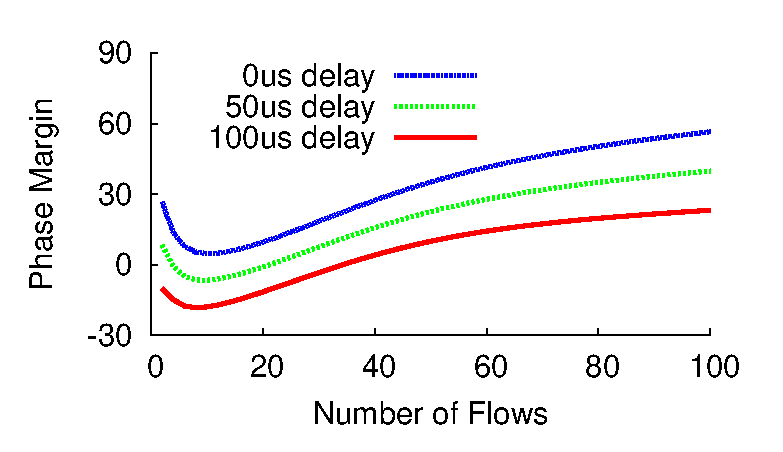
\includegraphics[width=0.33\textwidth]{figures/dcqcn_stability.eps}
\label{fig:dcqcn_stability_default}
}
\subfigure[DCQCN stability with $R_{AI}=10Mbps$.]
{
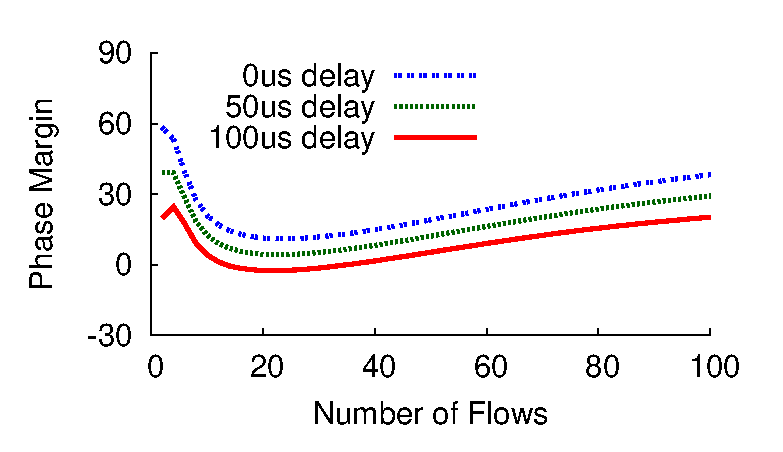
\includegraphics[width=0.33\textwidth]{figures/dcqcn_stability_rai.eps}
\label{fig:dcqcn_stability_rai}
}
\subfigure[[DCQCN stability with $R_{AI}=10Mbps$ and $K_{max}=1000KB$.]
{
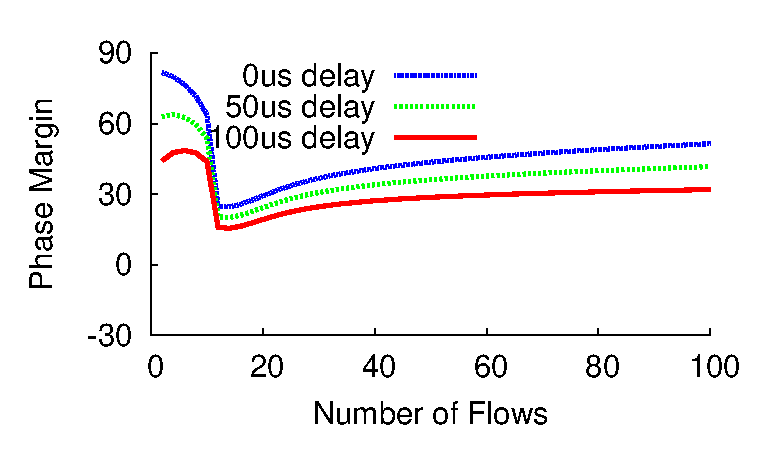
\includegraphics[width=0.33\textwidth]{figures/dcqcn_stability_rai_kmax.eps}
\label{fig:dcqcn_stability_rai_kmax}
}
\caption{DCQCN stability}
\label{fig:dcqcn_stability}
\end{figure*}

Below we show that DCQCN has a unique fixed point. We analyze DCQCN's stability around the 
fixed point, how stability varies under different conditions, and conclude with a 
parameter setting guideline.


\para{Fixed point.} By letting the left-hand side of Equation~\ref{eq:q}
be 0, it is easy to see that any of the fixed points (if exist) of DCQCN must satisfy:

\begin{equation}
\small
{R_C^*} = \frac{C}{N}
\end{equation}

At any of the fixed points, we assume the value of $p$ is $p^*$, then the queue length and
$\alpha$ at the fixed points are determined by Equation~\ref{eq:mark} and \ref{eq:alpha}:

\begin{equation}
\small
{q^*} = \frac{{{p^*}}}{{{p_{max}}}}\left( {{K_{max}} - {K_{min}}} \right) + {K_{min}}
\end{equation}
\begin{equation}
\small
\alpha^*  = 1 - {(1 - p^*)^{\frac{{\tau 'C}}{N}}}
\end{equation}

Next, we show that $p^*$ exists and is unique in the DCQCN model. 
From Equation~\ref{eq:rt} and \ref{eq:rc}, $R_T^*$ has two forms:

\begin{equation}
\small
{R_T^*} = \frac{C}{N} + \frac{{a\alpha }}{{(b + d)\tau }}
\end{equation}
\begin{equation}
{R_T^*} = \frac{C}{N}\left( {1 + \frac{{(c + e)\tau {R_{AI}}}}{a}} \right)
\end{equation}

Where we have the annotations of $a, b, c, d, e$, which have the value of following expressions
with $p(t) = p^*$.
\begin{equation}
\begin{array}{l}
a(t) = 1 - {(1 - p(t))^{\tau {R_C}(t)}},b(t) = \frac{{p(t)}}{{{{(1 - p(t))}^{ - B}} - 1}},\\
c(t) = \frac{{{{(1 - p(t))}^{FB}}p(t)}}{{{{(1 - p(t))}^{ - B}} - 1}},d(t) = \frac{{p(t)}}{{{{(1 - p(t))}^{ - T{R_C}(t)}} - 1}},\\
e(t) = \frac{{{{(1 - p(t))}^{FT{R_C}(t)}}p(t)}}{{{{(1 - p(t))}^{ - T{R_C}(t)}} - 1}}
\end{array}
\end{equation}

Combining the two forms of $R_T^*$, we see that the value of $p^*$ is determined by:
\begin{equation}
\small
\frac{{{a^2}\alpha }}{{(b + d)(c + e)}} = \frac{{{\tau ^2}{R_{AI}}C}}{N}
\label{eq:p_fixed}
\end{equation}

One can easily find that the left-hand side of the above equation is monotonic when $p \in [0,1]$.
When $p = 0$, the left-hand side of Equation~\ref{eq:p_fixed} is smaller than the right-hand side,
while is vice versa when $p = 1$. Thus DCQCN has a unique fixed point, determined by a unique $p^*$. 
Also, one can easily estimate the value of $p^*$ is very 
close to 0 using numerical approaches. Therefore, we can obtain the taylor series around $p=0$ of the left-hand side:

\begin{equation}
\small
\frac{{{a^2}\alpha }}{{(b + d)(c + e)}} = \frac{{{C^3}{\tau ^2}\tau '}}{{{N^3}{{\left( {\frac{1}{B} + \frac{N}{{CT}}} \right)}^2}}}{p^3} + O\left( {{p^4}} \right)
\end{equation}

Omitting the $O(p^4)$ term, combining Equation~\ref{eq:p_fixed}, we have the fixed point of $p$:

\begin{equation}
\small
{p^*} = \sqrt[3]{{\frac{{{R_{AI}}{N^2}}}{{\tau '{C^2}}}{{\left( {\frac{1}{B} + \frac{N}{{CT}}} \right)}^2}}}
\end{equation}

\para{Stability analysis.} 
We linearize the system by denoting $\delta {R_C}(t) = {R_C}(t) - R_C^*$, $\delta {R_C}(t) = {R_C}(t) - R_C^*$,
$\delta p(t) = p(t) - p^*$, $\delta \alpha (t) = \alpha (t) - \alpha^*$, and $A = \left( {\frac{1}{B} + \frac{1}{{TR_C^*}}} \right)$.
We further use Taylor series to simplify the expressions of $a, b, c, d, e$ to handle the exponential forms like $(1-p)^x$.
Because the equations are very complicated, here we just show an example of $R_C$. The linearized equation of $R_C$ is as follows:

\begin{equation}
\begin{array}{l}
\frac{{d\delta {R_C}}}{{dt}} =  - \frac{1}{2}{(R_C^*)^2}{\alpha ^*}\delta p - \frac{1}{2}{p^*}R_C^*{\alpha ^*}\delta R_C \\
 - \frac{1}{2}{p^*}R_C^*{\alpha ^*}\delta {R_C} - \frac{1}{2}{p^*}{(R_C^*)^2}\delta \alpha \\
 + \frac{A}{2}\left( {R_C^*\delta {R_T} - R_C^*\delta {R_C} + R_T^*\delta {R_C} - R_C^*\delta R_C} \right)\\
 - \left( {\frac{1}{2} + \frac{A}{4}} \right)\left( {{p^*}R_C^*\delta {R_T} - {p^*}R_C^*\delta {R_C} + {p^*}R_T^*\delta {R_C} - {p^*}R_C^*\delta R_C + R_C^*R_T^*\delta p - {{(R_C^*)}^2}\delta p} \right)
\end{array}
\end{equation}

We can then perform Laplace transform and get:

\begin{equation}
\small
\begin{array}{l}
s{R_C}(s) - \delta {R_C}(0) = \left( { - \frac{1}{2}{{(R_C^*)}^2}{\alpha ^*} - \left( {\frac{1}{2} + \frac{A}{4}} \right)R_C^*R_T^* + \left( {\frac{1}{2} + \frac{A}{4}} \right){{(R_C^*)}^2}} \right){e^{ - s\tau *}}p(s)\\
 + \left( { - \frac{1}{2}{p^*}R_C^*{\alpha ^*} - \frac{A}{2}R_C^* + \left( {\frac{1}{2} + \frac{A}{4}} \right){p^*}R_C^*} \right){e^{ - s\tau *}}{R_C}(s)\\
 + \left( { - \frac{1}{2}{p^*}R_C^*{\alpha ^*} - \frac{A}{2}R_C^* + \frac{A}{2}R_T^* + \left( {\frac{1}{2} + \frac{A}{4}} \right){p^*}R_C^* - \left( {\frac{1}{2} + \frac{A}{4}} \right){p^*}R_T^*} \right){R_C}(s)\\
 - \frac{1}{2}{p^*}{(R_C^*)^2}\alpha (s)\\
 + \left( {\frac{A}{2}R_C^* - \left( {\frac{1}{2} + \frac{A}{4}} \right){p^*}R_C^*} \right){R_T}(s)
\end{array}
\end{equation}

With Laplace tranform of the other equations, we can use ${R_C}(s)$ to express ${R_T}(s)$, $p(s)$ and $\alpha (s)$.
Then we can get the characteristic equation of ${R_C}(s)$. We test the characteristic equation against {\em Bode Stability
Criteria}. 

\begin{itemize}
\item DCQCN stability falls as the number of flow increases.
\item Smaller $R_{AI}$ leads to better stability.
\end{itemize}

\subsection{Convergence}
